\subsection{Actividad 3}
Obtener la función de transferencia en $z$ del sistema
servomotor de posición discretizado con $T=0.05$ (en bucle abierto) a
través de \textsc{MATLAB} y obtener la ecuación en diferencias
correspondiente.

Existen otros métodos para discretizar la planta pero solo podemos
usar el \textcolor{blue}{`zoh'} porque da el mejor resultado frente a
la reconstrucción del filtro de primer orden
(\textcolor{blue}{`foh'}).

\begin{tcolorbox}[sharp corners, colframe=bluebox, title= Función de
  transferencia en $z$.]
 $>>>$ Gposicionz = c2d(Gt,T,\textcolor{blue}{`zoh'})
  \vspace*{0.5em}
  \begin{tcolorbox}[sharp corners, colback = white]
    \color{gray}
\begin{verbatim}
Gposicionz =
 
  0.001609 z^2 + 0.003276 z + 0.0003034
  -------------------------------------
  z^3 - 1.801 z^2 + 0.8331 z - 0.03168
 
Sample time: 0.05 seconds
Discrete-time transfer function.
\end{verbatim}
  \end{tcolorbox}%
  \vspace*{0.5em}
\end{tcolorbox}%

Considerando el \textbf{sistema lineal discreto} descrito por la
ecuación en diferencias
\begin{equation}
  y(k+n) + a_1 \cdot y(k+n-1)+...+a_n \cdot y(k) = b_0 \cdot
  u(k+n)+...b_n\cdot u(k)
\end{equation}
con función de transferencia
\begin{equation}
  G(z) = \dfrac{Y(z)}{U(z)} = \dfrac{b_0 \cdot z^n + b_1 \cdot z^{n-1}
  + ... + b_n}{z^n+a_1 \cdot z^{n-1}+ ... + a_n}
\end{equation}
luego podemos usar esto para extraer la función.
\begin{equation}
  G(z) = \dfrac{Y(z)}{U(z)} = \dfrac{0.016 z^2+0.03231z+0.003004}{z^3-1.763z^2+0.7949z-0.03168}
\end{equation}
\begin{equation*}
  n = 3; \ b_1 = 0.0016; \ b_ 2 = 0.03231;\ b_3 = 0.003004;\ a_1 =
  -1.763;\ a_2 = 0.7949; \ a_3 = -0.03168
\end{equation*}
Con los parámetros anteriores podemos calcular la ecuación en
diferencias.
\begin{equation}
  y(k+3)-1.763y(k+2)+0.7949y(k+1)-0.03168y = 0.016u(k+2)+0.03231u(k+1)+0.003004u(k)
\end{equation}
Para confirmar que la conversión continua-discreta ha sido correcta
hemos representado ambas funciones de transferencia en una misma
gráfica, con un entrada impulso.
%\textcolor{red}{DUDA: Calcular la inversa mediante MATLAB o a mano}

\begin{tcolorbox}[sharp corners, colframe=bluebox, title= Funciones de
  transferencia.]
  $>>>$ figure\\
  $>>>$ step(Gposicion)\\
  $>>>$ hold \textcolor{blue}{on}\\
  $>>>$ step(Gposicionz)\\
  $>>>$ xlim([0 1])\\
  $>>>$ title(\textcolor{blue}{`Función de transferencia continua vs discreta.'})\\
  $>>>$ legend(\textcolor{blue}{`Función continua',`Función discreta'})\\
  $>>>$ grid \textcolor{blue}{on}\\
\mkanscode{
\begin{figure}[H]
  \centering
  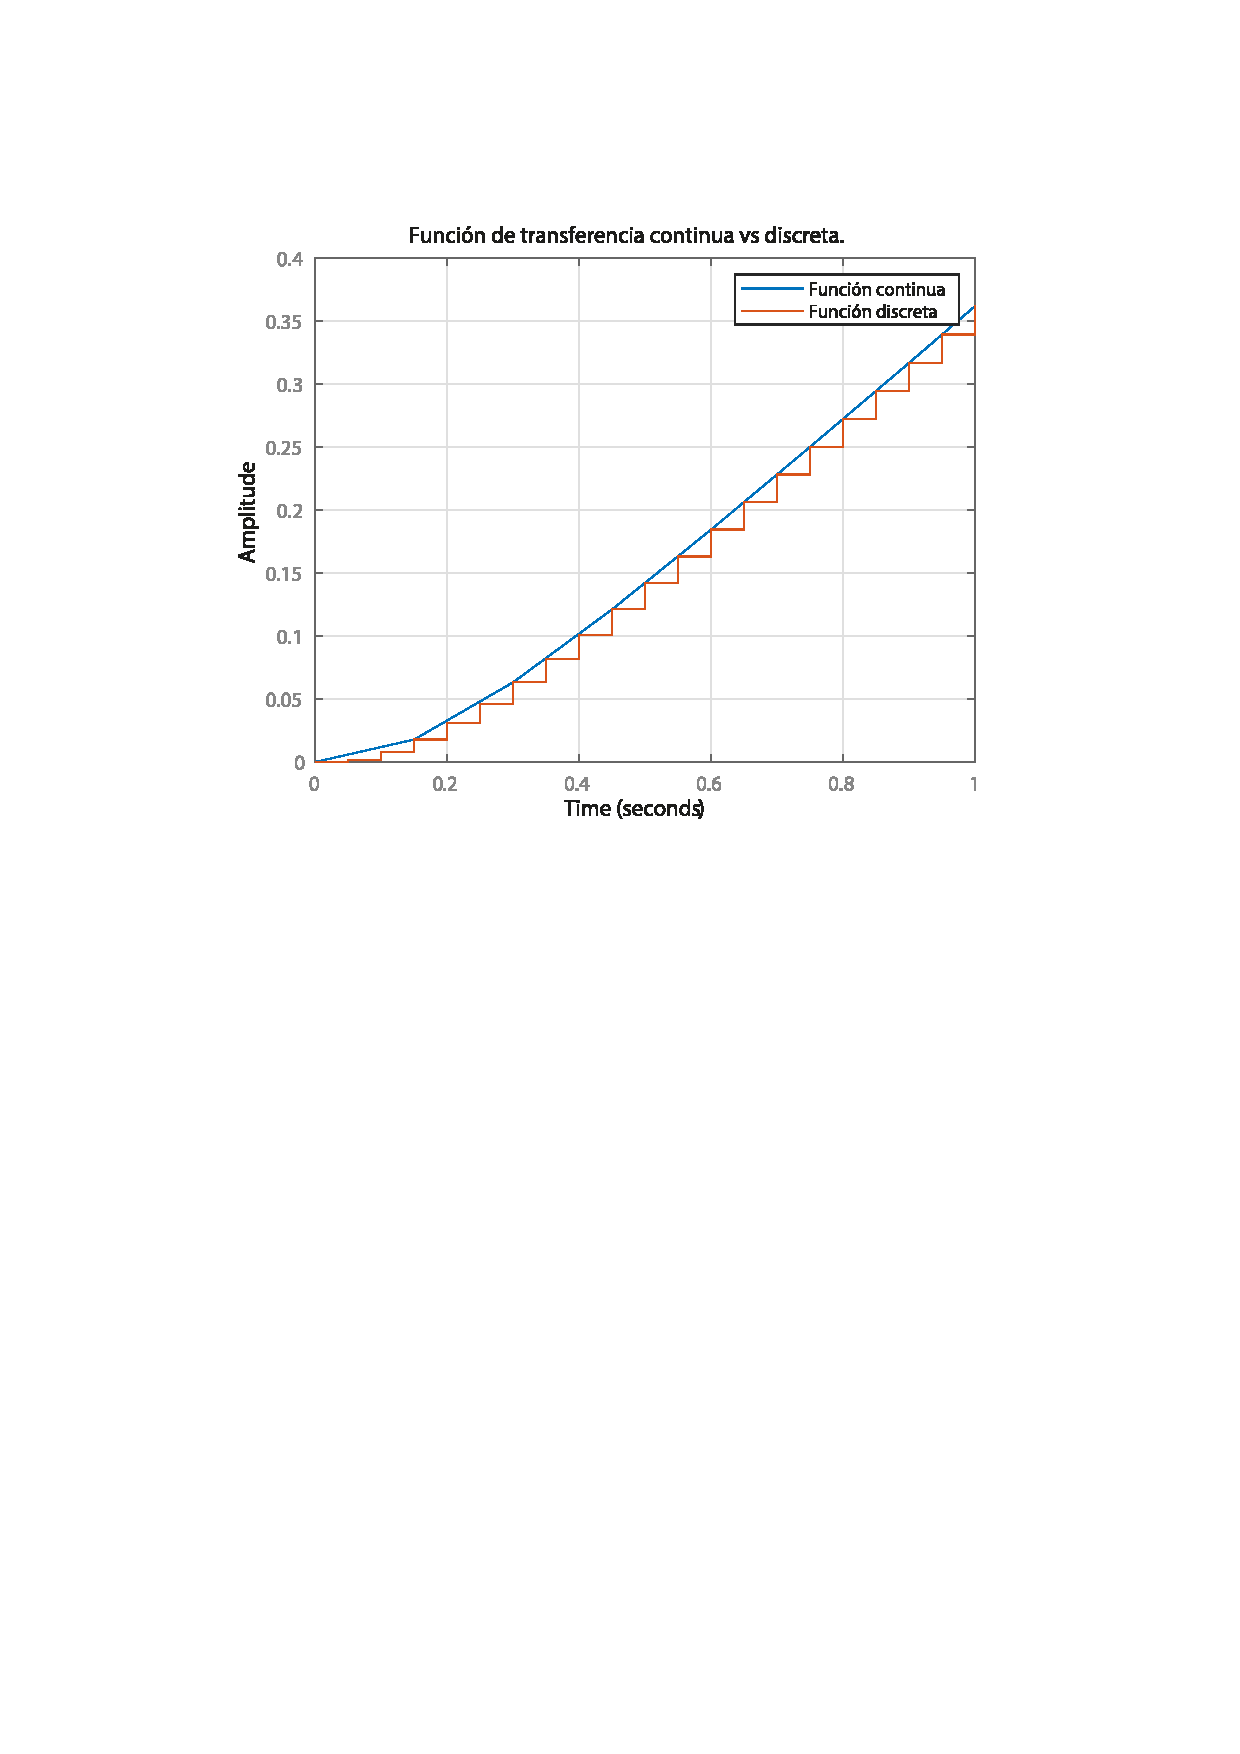
\includegraphics[clip, trim=3.5cm 15.5cm 2cm 3.5cm,
  scale=0.90]{images/figura 1.pdf}
  % izquierda,abajo,derecha,arriba
  \caption{Respuesta de funciones de transferencia frente a una
    rampa.}
    \label{fig:respuesta}
\end{figure}
}
\end{tcolorbox}%

